\documentclass[12pt,letterpaper]{article}
\usepackage[margin=1in]{geometry}
\usepackage{fancyhdr}
\usepackage[utf8]{inputenc}
\usepackage{palatino}
\usepackage{microtype}
\usepackage{hyperref}
\usepackage{graphicx}
\usepackage{lastpage}
\usepackage[hang,small]{caption}
\usepackage{titlesec}

\renewcommand{\headrulewidth}{0pt}
\fancyfoot{}
\fancyfoot[C]{\sffamily Page \thepage\ of \pageref{LastPage}} \pagestyle{fancy}

\titleformat{\section}{\bfseries\MakeUppercase}{\arabic{\thesection}}{1em}{}
\titleformat{\subsection}{\bfseries}{\arabic{\thesection}.\arabic{\thesubsection}}{1em}{}
\titleformat{\subsubsection}{\itshape}{\arabic{\thesection}.\arabic{\thesubsection}.\arabic{\thesubsubsection}}{1em}{}

\setlength{\parindent}{0cm}
\setlength{\parskip}{1em}

\captionsetup[figure]{labelfont=it,font=it}
\captionsetup[table]{labelfont={it,sc},font={it,sc}}

\hypersetup{colorlinks,
    linkcolor = black,
    citecolor = black,
    urlcolor  = black}
\urlstyle{same}



\begin{document}

\begin{center}
{
    \bfseries\huge
    Oregon State University \\
    Autonomous Aerial Robotics Team \\ [1em]
}
{
    \small
    Kyle Dillon, Daniel Miller, Tim Niedermeyer, Ryan Skeele, Michael Williams, Soo-Hyun Yoo \\ [0.5em]
    \emph{Oregon State University, Corvallis, OR 97330}
}
\end{center}

\begin{center}
\begin{minipage}{5.5in}

\section*{Abstract}

The Oregon State University Autonomous Aerial Robotics Team has developed an
indoor autonomous quadrotor with custom hardware and software to compete in the
International Aerial Robotics Competition (IARC). Onboard, an ATXmega128a3
microcontroller runs a 200 Hz PD orientation controller. The quadrotor is
capable of sending live video, LIDAR scans, and altitude measurements to the
base station which passes navigational commands back to the quadrotor. The
quadrotor possesses a passively compliant robotic hand that will be used to
pick up the USB flash drive in competition.

\end{minipage}
\end{center}


% TODO: Move to the end of the paper?
\begin{figure}[h!]
    % \includegraphics[width=6in]{teampic.png}
    \caption{Oregon State Aerial Robotics Team 2012}
\end{figure}


\section*{Introduction}

Our strategy for indoor automous flight involves specific functional goals for
each part of the system. Flight stability is handled by the flight platform,
however, all navigational data gathered from distance sensors and cameras
mounted on the flight platform is transmitted to the base station for
processing. The base station then transmits navigational commands to the flight
platform.

Stabilization sensory is handled using a three axis gyroscope, accellerometer
and magnetometer. Navigational data comes from a number of distance sensors
mounted on servos that act as an improvised LIDAR. This solution was chosen
because of the low electrical and computing power required to process distance
sensor data. A seperate wireless camera is implemented to provide object
recognition using the OpenCV libraries.


\section*{Hardware}

\subsection*{Chassis}

The new chassis design will make use of lighter weight carbon fiber tubing.
The current design consists of 4 motors mounted on arms that mount to a central
chassis. The new design will consist of only two solid arms that mount to one
another, each connecting a pair of motors. This will remove bending moments
resulting from motor forces from the central chassis, allowing for material
reduction and weight savings. The current chassis also has a tendency to snag
the ground when the aerial vehicle lands with significant lateral speed. This
causes the vehicle to tip over, sending its propellers into the ground and
causing damage. The new chassis will have less skid resistance, while allowing
for vertical impact absorption. Blade guards will also be added around the
perimeter of the propellers, to reduce the risk of propeller damage from
incidental contact with the environment.


\subsection*{End Effector}

The IARC competition requires the use of a grasping mechanism for one of the
primary objectives. The chosen design for the grasping mechanism will make use
of an under-actuated, passively compliant four-fingered hand. Each of the four
fingers will contain two flexure joints, rather than rotational bearing joints.
A fully actuated hand would require eight actuators; this under-actuated design
will require only one. A single actuator will control all joints through the
use of a pulley system, allowing each finger link to actuate until it comes
into contact with an object. All tendon cables will see the same force from
the actuator. Not only does this design greatly reduce cost, but it saves
weight--an essential benefit for an aerial vehicle. In addition, the design
all ows the hand to automatically adapt to the shape of any object, without the
need for special positioning and calculated movements.


\subsection*{Electronics}

\begin{figure}[h!]
    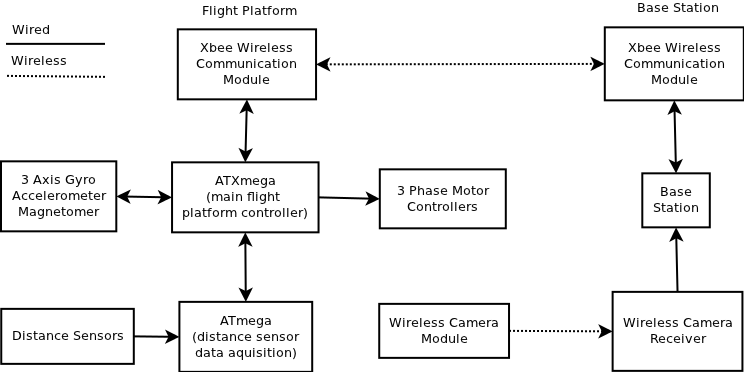
\includegraphics[width=6in]{controlhardware.png}
    \caption{Control Hardware Block Diagram}
    \label{fig:el_blockdia}
\end{figure}

A 3-cell lithium polymer battery powers the motors and motor controllers on the
quadrotor. The battery is also regulated down to 5 volts to power an Atmel
Xmega microcontroller used as the central intelligence on the flight platform,
a 2.4 GHz XBee radio for wireless communication, and various distance and
inertial sensors. The wireless camera is powered by a seperate 9 volt source. This system is illustrated in Figure~\ref{fig:el_blockdia}.


\section*{Software}

\subsection*{Aerial Stabilization and Flight Control}

% \section*{Flight Control} The on board flight control system was developed to
% provide basic stability for the flight platform. It does not have
% contingencies to prevent drift. Integration of gyroscope samples is used to
% create an estimate of the orientation of the flight platform. This combined
% with the raw data from the gyroscopes is as input to a position differential
% (PD) controller. To prevent the gyroscope positional estimates from drifting
% they are averaged with magnetometer and accelerometer samples.

\subsubsection*{Orientation Kinematics}

An accurate measurement of the aerial vehicle's orientation is key to
autonomous stabilization. The orientation can be represented with a direction
cosine matrix (DCM), which is a 3x3 matrix containing the cosines between each
of the 9 possible pairs of axes of two separate Cartesian coordinate systems.

In the context of inertial measurement units in robotics applications, a 3D
vector could be represented in either the global (earth) or the body (local)
frames of reference. For example, the location of an end effector may be
represented as $\langle1, 0, 0\rangle$ in the body frame but have different and
changing X, Y, and Z components in the global frame, and vice versa.

If the controller loop frequency is high enough (on the order of 100 Hz), an
axis of the DCM, its rotational vector, and its linear velocity are
approximately orthogonal to each other. Thus, the magnitude of the angular
velocity of a unit vector approximately equals its linear velocity, which means
that the DCM can be calculated by integrating the gyroscope readings.

Unfortunately, since the gyroscope only measures the change in the orientation,
the DCM will drift over time. A 3-axis accelerometer can be used to correct the
roll and pitch drift. A 3-axis magnetometer to correct for yaw drift. Between
those two sensors, an accurate DCM can be maintained.

%In order to achieve this, we wish to keep the calculated global Z vector
%codirectional with the negative gravity vector. That is, the cross product of
%the two vectors should equal zero, and we can use whatever the cross product
%actually is as our correctional rotation vector. It is important to keep in
%mind, however, that since the accelerometer reports acceleration in the body
%frame of reference, we must express Z in the same frame of reference as the
%acceleration vector.

%This body frame Z vector is simply found by taking the third row of the
%transpose of the DCM. We cross multiply Z with the gravity vector, add the
%resulting correction vector to the angular displacement vector, and take a
%weighted average.

%Small imperfections in the mounting of the accelerometer can be offset by a
%rotation matrix.


\begin{figure}[h!] 
\includegraphics[width=6in]{posterbackground_cropped.png}
\caption{Prototype Flight Platform Operating Outdoors}
\end{figure}



\subsubsection*{Cascading PID Controllers}

The D controller in a simple angular position PD controller can hinder the
responsiveness of the quadrotor, which is crucial to stability. A better
alternative is an angular position P controller that feeds a desired velocity
to an angular velocity PD controller.

At first thought, it might seem that this combination of a position P
controller and a velocity PD controller is no different than a position PD
controller, since both the position D and the velocity P are based on velocity
measurements. However, the two controllers do different things with the
velocity measurements.

The position D controller has a damping effect on motion in that it always
resists a change in position. This means that if the quadrotor experiences a
perturbation away from some desired position, the D controller will help resist
the motion, as desired. However, as the quadrotor tries to recover from this
error state, the D controller blindly hinders the movement back towards the
desired position, which is not at all optimal.

The velocity P controller, on the other hand, pushes the velocity to whatever
it should be, whether that means slowing it down or speeding it up. The
velocity D controller ensures that the velocity change does not happen too
abruptly, helping reduce the chance of overshoot. The controller is able to do
this by keeping track of a desired velocity in addition to the current
velocity, which provides a context upon which the controller can ``decide''
whether it should help a positional movement or hinder it, instead of blindly
hindering all movement as is the case with a position D controller.

This means that the P/PD controller as a whole can take a desired position
input and accelerate the body towards and maintain a target angular velocity
until the current position nears the target position. Only then will the
controller actively slow down the movement. This makes for a controller that
can respond much more quickly while maintaining stability.

\subsection*{Navigation}
\subsubsection*{Navigation Hierarchy}
	Our navigation hierarchy modularizes each part of our system to have a
specific set of responsibilities with little overlap. The intelligence contained
on the flight platform is solely responsible for maintaining a stable
orientation. Additionally the flight platform forwards navigational data from
distance sensors through xbee radios and images from a wireless camera using the
camera's own self contained wireless transmission capabilities. Navigation data is processed on the base station, which is responsible
for completing the mission. It sends commands back to the flight platform based
on the navigational data it has received.

\subsubsection*{Navigation Strategy}
	In order to navigate indoor environments we implement an array of simple
distance sensors, some mounted on pan or tilt mechanisms, to act as an
improvised LIDAR system. This approach was chosen because of its accesibility,
low power, and low bandwidth requirements.
	Distance sensor data gathered on the flight platform is not processed
there and instead forwarded to the base station. The base station operates
using Robot Operating System, which processes both distance sensor data and
images sent from the fligh platform to make navigational decisions. These
decisions are then relayed back to the flight platform as movement commands.

\end{document}
